\subsubsection{Energy Loss Correction}\label{section:star_energyLoss}
Particles passing through the detector material lose energy on their way. The track transverse momentum $p_\textrm{T}$ is reconstructed by fitting a helical path to the~hits. Fitting the track points to an ideal
helical track tends to underestimate the momentum due to energy loss. To minimize biases due to this effect, a~correction procedure is applied 
during standard track momentum reconstruction. For this procedure pion hypothesis is used  and the reconstructed momentum $p_\textrm{T}^\textrm{meas}$ is corrected by the amount of energy loss specific for a pion.  For all particles but a pion some rest bias  is still present since  energy loss is specific for each particle type. 
The correction $p_\textrm{T}^\textrm{meas}-p_\textrm{T}^\textrm{true}$ due to these biased was determined from MC for each particle species as a function of $p_\textrm{T}^\textrm{meas}$, $\eta$ and $V_z$. 
The sample energy loss correction averaged over $|\eta|<0.7$ for $K^-$ and $\bar{p}$ are shown in Fig.~\ref{fig:energyLoss}. 

\begin{figure}[h!]
	\centering
	\includegraphics[width=0.49\textwidth,page=30]{chapters/chrgSTAR/img/energyLoss/energyLoss3D_OnePrtAlso.pdf}
	\includegraphics[width=0.49\textwidth,page=50]{chapters/chrgSTAR/img/energyLoss/energyLoss3D_OnePrtAlso.pdf}
		\caption{Sample energy loss correction $p_\textrm{T}^\textrm{meas} - p_\textrm{T}^\textrm{true}$ for (left) $K^-$ and (right) $\bar{p}$ as a function of reconstructed transverse 
			momentum $p_\textrm{T}^\textrm{meas}$ ($|\eta| < 0.7$) in single $z$-vertex bin, $-10 < V_z < 0$~cm. Red lines and arrows indicate region 
			accepted in analysis.}
		\label{fig:energyLoss}
	
\end{figure}



